% ///////////////////////////////////////////// %
% /// Les types de bases de données NoSQL ///// %
\section{Les types de bases de données NoSQL}

	%% Bases de données clé-valeur
	\subsection{Bases de données clé-valeur}
	\begin{frame}
		\frametitle{Modélisation BD clé-valeur}

		\begin{itemize}
			\item \textbf{Modélisation :} la plus simple. À une clé, on associe une valeur. La valeur peut être de n'importe quel type (chaîne de caractères, entier, structure, objet sérialisé\dots).
		\end{itemize}

		\vspace{15px}
		Des exemples de paires clé-valeur avec des types différents.
		\vspace{5px}
		\begin{tabular}{|l|l|}
			\hline
			\textbf{Clé} & \textbf{Valeur} \\ \hline\hline
			pays.id-42 & \{"id":42,"name":"Chad"\} \\ \hline
			statistiques.nombre-visiteurs & 1337 \\ \hline
			configuration.periode-gratuite & false \\ \hline
			articles.categories-sport.latest & [22, 45, 67, 200, 87] \\ \hline
		\end{tabular}
	\end{frame}

	\begin{frame}
		\frametitle{BD clé-valeur en détail}
		\begin{itemize}
			\item \textbf{Opérations} : création d'une paire clé-valeur, suppression, accès à une valeur à l'aide de la clé, incrémentation et décrémentation d'une valeur ;
			\item Stockage en RAM pour accélérer les temps de lecture. Mécanisme de reprise en cas de crash ;
			\item On peut définir la durée de vie d'une paire clé-valeur ou adopter une politique \textit{least recently used} ;
			\item \textbf{Cas d'utilisation :} cache d'une autre BD, comptage d'éléments, gestion de files d'attente, opérations ensemblistes\dots
			\item \textbf{Principaux acteurs :} Redis, Memcached, Riak.
		\end{itemize}
	\end{frame}

	\begin{frame}
		\frametitle{Commandes sous Redis}

		\begin{listing}[H]
			\inputminted[fontsize=\tiny, linenos=true]{text}{code/commandesRedis.txt}
			\caption{Quelques commandes Redis en console.}
		\end{listing}

	\end{frame}

	%% Bases de données document
	\subsection{Bases de données orientées documents}
	\begin{frame}
		\frametitle{Bases de données orientées documents}

		\begin{itemize}
			\item \textbf{Modélisation :} aucun schéma fixe, un document peut contenir n'importe quel type d'information ;
			\item \textbf{Opérations :} utilise le JSON pour les requêtes et l'améliore pour le stockage (BSON) ;
			\item \textbf{Cas d'utilisation :} base de données principalement utilisées pour du stockage ;
			\item \textbf{Avantages :} facile d'accès et optimisation horizontale ;
			\item \textbf{Principaux acteurs :} MongoDB, CouchDB, CouchBase.
		\end{itemize}

	\end{frame}

	\begin{frame}
		\frametitle{Exemple d'un document}

		\begin{listing}[H]
			\inputminted[fontsize=\tiny, linenos=true]{json}{code/exemple-document.json}
			\caption{Exemple d'un document JSON.}
		\end{listing}
	\end{frame}

	\begin{frame}
		\frametitle{Exemples de requêtes MongoDB}


		\begin{exampleblock}{Base de données MongoDB au quotidien}
			De nombreux acteurs proposent la visualisation et l'exécution de requêtes sur une base de données MongoDB : le shell Mongo, Robomongo, PHPMoAdmin\dots 
		\end{exampleblock}


	\end{frame}


	%% Bases de données graphe
	\subsection{Bases de données orientées graphes}
	\begin{frame}
		\frametitle{Bases de données orientées graphes}

		\begin{figure}[htb]
			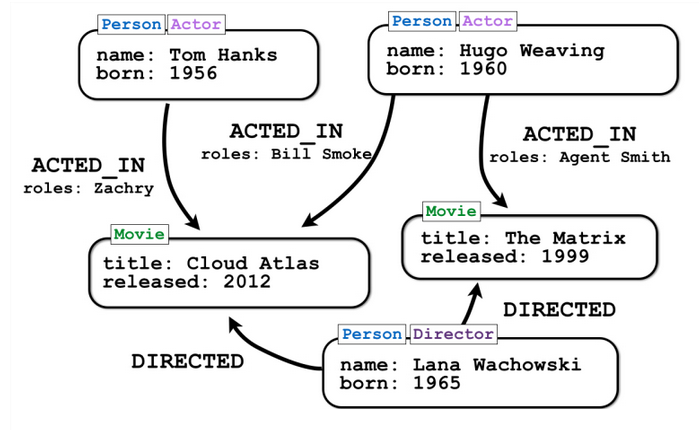
\includegraphics[width=1\textwidth]{images/graphe.png}
			\caption{Exemple de graphe.}
		\end{figure}

	\end{frame}

	\begin{frame}
		\frametitle{Exemple de requête}

		\begin{figure}[htb]
			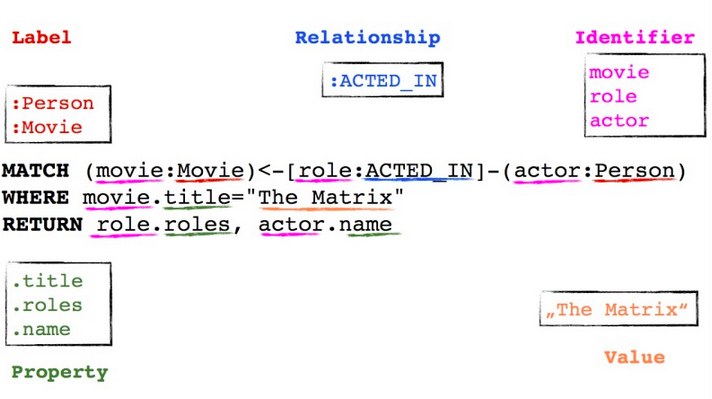
\includegraphics[width=1\textwidth]{images/requeteNeo4j.png}
			\caption{Exemple de requête Cypher pour Neo4j.}
		\end{figure}

	\end{frame}

	\begin{frame}
		\frametitle{Bases de données orientées graphes}

		\begin{itemize}
			\item \textbf{Modélisation :} représentation de l'information de manière très particulière (nœuds et arcs de même importance) ;
			\item \textbf{Cas d'utilisation :} utilisé principalement pour les réseaux (liens entre des équipements ou des personnes) ;
			\item Base de données rarement utilisée pour du stockage ;
			\item \textbf{Opérations :} traitement très particulier de l'information (voir slide précédente) ;
			\item \textbf{Principaux acteurs :} Neo4j, Titan, OrientDB.
		\end{itemize}

	\end{frame}